\documentclass[twoside]{article}
\usepackage[utf8]{inputenc}
\usepackage{amsmath,amsfonts,amssymb,amsthm,latexsym}
\usepackage[spanish,es-noshorthands]{babel}
\usepackage[T1]{fontenc}
\usepackage{lmodern}
\usepackage{graphicx,hyperref}
\usepackage{tikz,pgf}
\usepackage{marvosym}
\usepackage{multicol}
\usepackage{fancyhdr}
\usepackage[papersize={5.5in,8.5in},left=.75cm,right=.75cm,top=1.5cm,bottom=1.25cm]{geometry}
\usepackage{fancyhdr}
\pagestyle{fancy}
\fancyhead[LE]{Colegio Arborizadora Baja}
\fancyhead[RE]{PEI:``Hacia una cultura para el desarrollo sostenible''}
\fancyfoot[RO]{\Email iedabgerman@autistici.org}
\fancyhead[LO]{\url{www.autistici.org/mathgerman}}
\fancyfoot[RE]{\Email cedarborizadoraba19@redp.edu.co}
\fancyfoot[LE]{Calle 59I \#44A - 02 \Telefon 7313994 - 7313995}
\fancyhead[RO]{Nit 830024976-8, Código DANE 11100103084-8}

\author{Germ\'an Avenda\~no Ram\'irez~\thanks{Lic. Mat. U.D., M.Sc. U.N.}}
\title{\begin{minipage}{.2\textwidth}

\includegraphics[height=1.75cm]{Images/logo-colegio.png}\end{minipage}
\begin{minipage}{.55\textwidth}
\begin{center}
Números racionales $\mathbb{Q}$ II\\
Matemáticas $9^{\circ}$
\end{center}
\end{minipage}\hfill
\begin{minipage}{.2\textwidth}

\includegraphics[height=1.75cm]{Images/logo-sed.png} 
\end{minipage}}
\date{}
\thispagestyle{plain}
\begin{document}
\maketitle
Nombre: \hrulefill Curso: \underline{\hspace*{44pt}} Fecha: \underline{\hspace*{2.5cm}}
%\begin{minipage}{.95\textwidth}
%\fbox{\textit{No raye ni dañe esta hoja para que pueda usarla otro compañero}}
%\end{minipage}
\section*{Continuación nivel II}
\begin{enumerate}
\item Efectúe ordenadamente las siguientes operaciones:
\begin{enumerate}
\item $\left[\dfrac{1}{4}+\dfrac{1}{3}\left(\dfrac{1}{3}-\dfrac{1}{6}\right)\right]-\left[2\div \left(\dfrac{2}{5}+1\right)\right]\cdot 3$
\item $\dfrac{1}{2}-\dfrac{1}{2}\left[1+\dfrac{1}{2}\left(\dfrac{1}{2}-1\right)-\dfrac{1}{2}\right]$
\item $\dfrac{1}{5}-22\div \dfrac{10}{3}+3\left(1-\dfrac{2}{5}\right)-\left(\dfrac{3}{5}-\dfrac{2}{3}\right)$
\end{enumerate}
\item Calcule y simplifique todo lo que sea posible:
\begin{enumerate}
\item $-2+\dfrac{1}{2}\left\{2+\dfrac{1}{2}\left[2+\dfrac{1}{2}\left(2+\dfrac{1}{2}\right)\right]\right\}$
\item $\dfrac{\left(\frac{1}{3}-1\right)+2\left(5-\frac{1}{2}+2\div \frac{1}{3}-7\right)}{1+\frac{5}{2}\left(\frac{3}{4}-\frac{1}{6}\right)-2+\frac{1}{3}}$
\end{enumerate}
\item ¿A qué númer entero es igual cada una de estas potencias?
\begin{enumerate}
\begin{multicols}{3}
\item $1^{-37}$
\item $(-1)^{-7}$
\item $\left(\dfrac{1}{2}\right)^{-2}$
\item $\left(-\dfrac{1}{2}\right)^{-4}$
\item $\left(-\dfrac{1}{3}\right)^{-2}$
\item $\left(\dfrac{4}{5}\right)^{0}$
\end{multicols}
\end{enumerate}
\item Un chico sale de marcha y gasta primero los 2/5 de su dinero y luego 1/6 de lo que le quedaba. Si regresa con \$3.900. ¿Con cuánto dinero salió?
\item Una agencia propone un viaje a un grupo de empleados de una oficina. Inicialmente interesa el viaje a una octava parte de la plantilla. Cuando se concreta el precio se retiran 3/5 de los que pensaban ir. Por causas diversas, una semana antes se retiran 1/21
de los que quedaban. Si al final van 80 personas. ¿Cuántas personas forman parte de la plantilla de la oficina?
\item Un vaquero se dirige desde Fort Smith a James City. El 34\% de este trayecto lo recorre en tren y las dos terceras partes de lo queda en una carreta. El resto a caballo. ¿Qué
tanto por ciento recorre a caballo? Si la distancia total son 360 millas. ¿Cuántas recorre a caballo?
\item Escriba tres números decimales comprendidos entre:
\begin{enumerate}
\begin{multicols}{2}
\item $-4,28$ y $-4,1$
\item $5,4$ y $5,4444\ldots$
\item $-3,5666\ldots$ y $-3,5$
\item $1,7856$ y $1,785656\ldots$
\end{multicols}
\end{enumerate}
\item Escribe dos fracciones tales que:
\begin{enumerate}
\begin{multicols}{2}
\item $\dfrac{18}{13}>\dfrac{a}{b}>\dfrac{c}{d}>\dfrac{17}{13}$
\item $0,36<\dfrac{x}{y}<\dfrac{y}{w}<0,3636\ldots$
\end{multicols}
\end{enumerate}
\item Escriba en forma de potencia la relación que existe entre los números de cada expresión:
\begin{enumerate}
\begin{multicols}{2}
\item $\sqrt[3]{8}=2$ $\Longleftrightarrow$ $2^{3}=8$
\item $\sqrt[5]{3125}=5$
\item $\sqrt[6]{4096}=4$
\item $\sqrt[4]{6561}=9$
\end{multicols}
\end{enumerate}
\item Calcule:
\begin{enumerate}
\begin{multicols}{3}
\item $32^{1/5}$
\item $81^{1/4}$
\item $2.187^{1/7}$
\end{multicols}
\end{enumerate}
\item Obtenga con la calculadora el valor aproximado a 4 cifras decimales de las siguientes raíces:
\begin{enumerate}
\begin{multicols}{3}
\item $\sqrt[3]{100}$
\item $\sqrt[5]{245}$
\item $\sqrt{0,5}$
\end{multicols}
\end{enumerate}
\item Escriba en notación científica:
\begin{enumerate}
\item $73.256''000.000'000.000$
\item La centésima parte de una diezmilésima
\item $0,0000002$
\item $0,00000000425$
\end{enumerate}
\item Exprese en notación científica las siguientes magnitudes:
\begin{enumerate}
\item Peso de un grano de arroz: 0,000027 kg.
\item Número de granos de arroz en un kilogramo: 36000 granos.
\item Número de moléculas que hay en un gramo de hidrógeno:\\ 301.000.000.000.000.000.000.000 moléculas.
\end{enumerate}
\item Efectúe con la calculadora y escriba el resultado con todas las cifras:
\begin{enumerate}
\item $5,2\cdot 10^{11}-1,2\cdot 10^{12}+7,2 \cdot 10^{12}$
\item $4,2\cdot 10^{-6}-8,2\cdot 10^{-7}+1,8\cdot 10^{-5}$
\item $(2,25\cdot 10^{22})\cdot (4\cdot 10^{-15}\div (3\cdot 10^{-3})$
\end{enumerate}
\item Calcule el número aproximado de glóbulos rojos que tiene una persona, sabiendo que tiene unos 4.500.000 por milímetro cúbico de sangre, y que su cantidad de sangre es de 5 litros. Exprésalo en notación científica.\\Calcule la longitud que ocuparían esos glóbulos rojos puestos en fila, si su diámetro es 0,008 milímetros por término medio.
\end{enumerate}
\section*{Nivel III}
\begin{enumerate}
\item Efectúa las siguientes operaciones con números enteros:
\begin{enumerate}
\item $5-[-(-4+6)-(-3+2)-(-2+4)]-(-3+4)-[-(-3+6)-2]$
\item $\left\{\dfrac{[(8-7+15)-6]\cdot (-4)}{(-5)\cdot [(-7+13-8)-(-1)]}\right\}\div [(-5+4)\cdot (13-15)]$
\end{enumerate}
\item Tres toneles, cuyas capacidades son 250, 306 y 504 litros están llenos de diferentes clases de vino. Se quieren envasar, sin mezclar, en botellas iguales. Halla la capacidad máxima que pueden tener estas botellas, y el número de botellas necesarias para proceder al envasado.
\item ¿Cuántos músicos, como mínimo, hay en una banda de música que cuando desfila de dos en dos sobra uno, y también sobra uno si desfilan de tres en tres, de cuatro en cuatro y de cinco en cinco?
\item Exprese en forma de fracción las partes coloreadas de las siguientes figuras:
\begin{enumerate}
\begin{multicols}{3}
\item 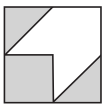
\includegraphics[scale=.8]{Images/Pantallazo-48.png}
\item 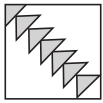
\includegraphics[scale=.8]{Images/Pantallazo-49.png} 
\item 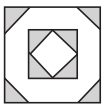
\includegraphics[scale=.8]{Images/Pantallazo-50.png} 
\end{multicols}
\end{enumerate}
Efectúa ordenadamente las siguientes operaciones:
\begin{enumerate}
\begin{multicols}{2}
\item $\dfrac{1-\dfrac{1-\frac{1}{3}}{1+\frac{1}{3}}}{1+\dfrac{1+\frac{1}{3}}{1-\frac{1}{3}}}-\dfrac{1}{6}$
\item $\dfrac{\left[\frac{3}{5}-\frac{2}{21}\left(-\frac{1}{5}-\frac{19}{20}\right)\right]\cdot \frac{3}{5}}{1-\dfrac{2}{1-\frac{1}{9}}}$
\end{multicols}
\end{enumerate}
\item Una señora sale de paseo y se encuentra a un pobre, al cual le da la mitad del dinero que lleva más una peseta. Se encuentra a otro pobre, al que le da la mitad del dinero que le quedaba más dos pesetas. Finalmente, al tercer pobre que le pide limosna le da
la mitad de lo que le quedaba más tres pesetas. En su monedero le quedó una peseta. ¿Cuánto dinero tenía antes de salir?
\item Un vendedor ambulante lleva una cesta de naranjas. En la primera casa que visita vende la mitad de las naranjas que lleva más media naranja. En la segunda vende la mitad de las que le quedaban más media. En la tercera y en la cuarta casa repite la
misma operación, con lo que se le agota la mercancía. ¿Cuántas naranjas llevaba al principio?
\item En una banda municipal de música, el 16,66666...\% de los miembros son trompetas y el 22,22222...\% son tambores. Además, se sabe que el número de músicos no llega a 40, aunque sobrepasa los 30. ¿Cuántas personas forman la banda?
\item Los 16 estados miembros de la OTAN dedicaron en el año 1995 unas $6,5 \cdot 10^{13}$ pesetas\footnote{La peseta es la moneda usada en España} a gastos de defensa, lo que supone un 4,1\%, como media de su Producto Interior Bruto (PIB). Expresa, en notación científica y en billones de pesetas el PIB de los países de la OTAN. (En nuestra lengua, 1 billon $=10^{12}$ , 1 trillón $= 10^{18}$)
\item El cabello humano crece, aproximadamente, un cm. en un mes. ¿Cuánto crece en una hora?
\item A las 4 de la tarde del 11-6-92, en la Cumbre de la Tierra de Río de Janeiro, un reloj digital con dos pantallas reflejaba la grave situación de la población mundial.\\
La primera pantalla marcaba el número de habitantes de la tierra: $5 4 6. 7 1 7 . 6 7 0$. Cada segundo, esa cifra aumentaba en 7 unidades, cantidad de niños que nacen en ese tiempo.\\
La segunda marcaba el número de hectáreas de tierra cultivable que hay en la Tierra: $8 7 2 . 2 7 2 . 2 4 2$
Cada 8 segundos, esa cifra disminuía en una unidad, ritmo al que se destruyen las tierras cultivables.
\begin{enumerate}
\item Si quieres recordar cuál es aproximadamente la población mundial, ¿qué cifra memorizarías?
\end{enumerate}
\end{enumerate}
\end{document}
